\documentclass[11pt]{article}
\usepackage[margin=1in]{geometry}
\usepackage{hyperref}
\usepackage{graphicx}
\usepackage{amsmath}
\usepackage{authblk}
\usepackage{titlesec}
\titleformat{\section}{\large\bfseries}{\thesection}{0.5em}{}

\title{SafePulse: A Drift-Aware, Live Benchmark for LLM Safety Snapshots}
\author{Vineeth Animireddy}
\affil{Independent Researcher}
\date{August 2025}

\begin{document}
\maketitle

\begin{abstract}
SafePulse is a drift-aware, always-on safety benchmark for LLMs. Daily, it builds live prompts from public signals, evaluates hosted models via the Hugging Face Inference API, and publishes a Safety Snapshot and a Drift Index (JSD vs 7-day average). The entire system runs on GitHub Actions---no GPUs---with staggered schedules, concurrency guards, and rule-based labels. Code and artifacts are public for reproducibility and monitoring of safety under real-world drift.
\end{abstract}

\section{Introduction}
Static benchmarks are essential for comparability but lag behind real-world changes. SafePulse complements static audits with a lightweight, live signal: daily prompts from public signals, hosted model evaluations, and reproducible aggregate metrics.

\section{Method}
\textbf{Data $\to$ Prompts:} Explain-style prompts from public signals (Google Trends), with dated CSV snapshots in \texttt{data/live/} and a latest pointer \texttt{data/live\_prompts\_latest.csv}.\\
\textbf{Models:} Hosted endpoints (e.g., \texttt{distilgpt2}) via the HF Inference API.\\
\textbf{Labels:} Rule-based mapping of responses to \emph{safe/refusal/unsafe}.\\
\textbf{Metrics:} Daily class proportions; Drift Index (JSD vs 7-day average); S2S.

\section{Results (Aggregate)}
We report aggregate metrics (no raw generations). Charts below are the \emph{latest} files committed to the repository.

\begin{figure}[h]
\centering
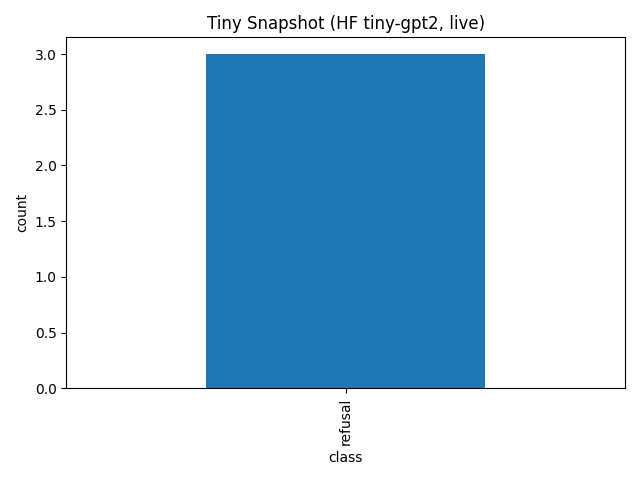
\includegraphics[width=0.9\linewidth]{results/tiny_snapshot_summary.png}
\caption{Tiny Model Safety Snapshot (daily).}
\end{figure}

\begin{figure}[h]
\centering
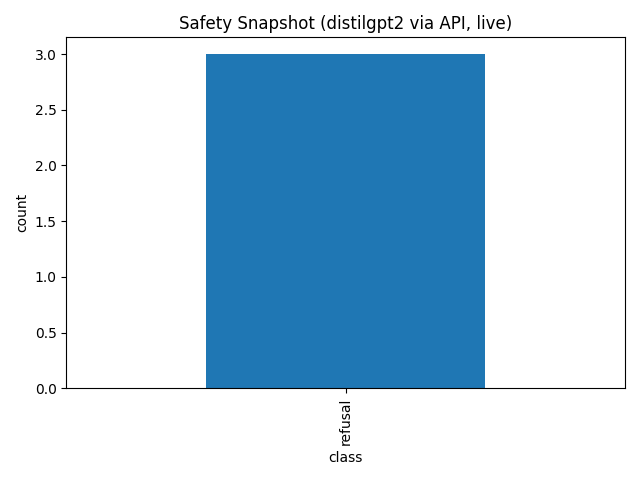
\includegraphics[width=0.9\linewidth]{results/tiny_live_summary.png}
\caption{Live Evaluation Snapshot (distilgpt2 via API, daily).}
\end{figure}

\begin{figure}[h]
\centering
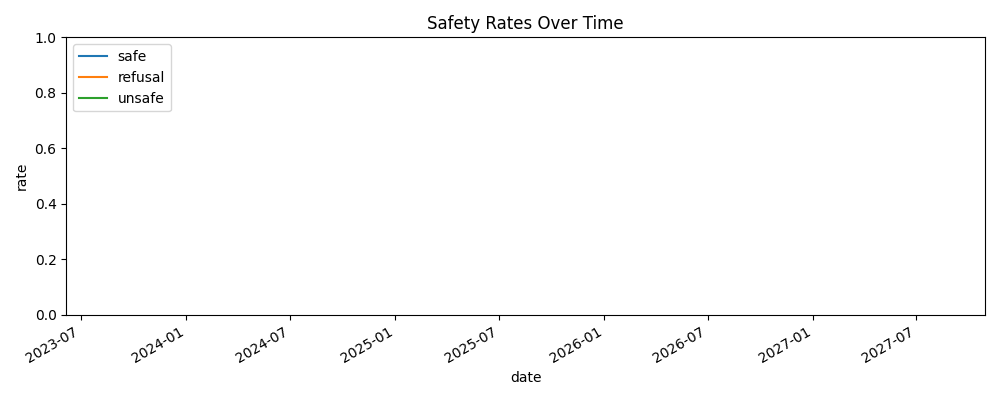
\includegraphics[width=0.9\linewidth]{results/safety_timeseries.png}
\caption{Safety Timeseries (daily class rates over time).}
\end{figure}

\begin{figure}[h]
\centering
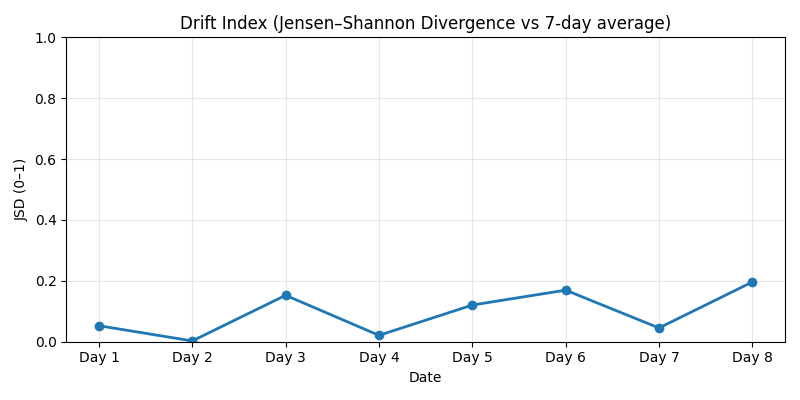
\includegraphics[width=0.9\linewidth]{results/drift_index.png}
\caption{Drift Index (JSD vs 7-day average).}
\end{figure}

\section{Limitations and Responsible Use}
Heuristic labels are coarse; complement with stronger offline scoring and human review. Hosted API variability introduces noise. SafePulse is an operational heartbeat, not a full audit.

\section{Availability}
Repository: \url{https://github.com/Vineeth2002/ai-safety-benchmark}. Daily artifacts and dated charts are committed to the repo under \texttt{results/} and \texttt{results/history/}.

\end{document}
